\begin{figure}[ht]
\centering
\scalebox{0.65}{%
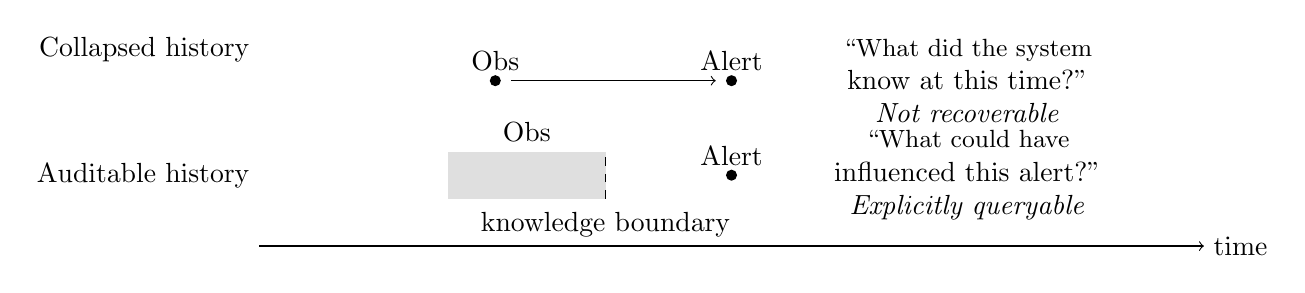
\begin{tikzpicture}[x=1cm,y=1cm]

% Time axis
\draw[->] (0,0) -- (12,0) node[right]{time};

% Labels
\node[anchor=east] at (0,2.5) {Collapsed history};
\node[anchor=east] at (0,0.9) {Auditable history};

% ---- Collapsed history ----
% Events
\fill (3,2.1) circle (2pt);
\node[above] at (3,2.1) {Obs};

\fill (6,2.1) circle (2pt);
\node[above] at (6,2.1) {Alert};

% Arrow
\draw[->] (3.2,2.1) -- (5.8,2.1);

% Annotation
\node[align=center] at (9,2.1)
  {\small ``What did the system\\know at this time?''\\\textit{Not recoverable}};

% ---- Auditable history ----
% Observation interval
\draw[fill=gray!25,draw=none] (2.4,0.6) rectangle (4.4,1.2);
\node[above] at (3.4,1.2) {Obs};

% Alert point
\fill (6,0.9) circle (2pt);
\node[above] at (6,0.9) {Alert};

% Knowledge window
\draw[dashed] (4.4,0.6) -- (4.4,1.2);
\node[below] at (4.4,0.55) {knowledge boundary};

% Annotation
\node[align=center] at (9,0.9)
  {\small ``What could have\\influenced this alert?''\\\textit{Explicitly queryable}};

\end{tikzpicture}
}
\caption{Auditability under collapsed versus propagated time. \conceptual\; When timestamps are rewritten or normalised (top), historical system state cannot be reconstructed; when temporal uncertainty is preserved (bottom), the system retains an explicit boundary between what was known and what was not, enabling post-hoc audit, explanation, and governance.}
\end{figure}